\documentclass[a4paper,UTF8]{ctexart}

% Author affiliation
\usepackage{authblk}
% Package for line spacing
\usepackage{setspace}
\renewcommand{\baselinestretch}{2.0} % Double spacing
% Margins
\usepackage[margin=1.25in]{geometry}
% Mathematics
\usepackage{amsmath}
% Tables
\usepackage{tabularx}
\usepackage{booktabs}
% SI units
\usepackage{siunitx}
% Links and referencing within the document
\usepackage[backref]{hyperref}
\hypersetup{hidelinks} 
% Advanced math typesetting
\usepackage{mathtools}
% Graphics
\usepackage{graphicx}
\usepackage{subfig} 
\graphicspath{{./figures}} % Adjust path as needed

\title{这只是一个示例}

\author[1$\dag$]{X}
\author[1$\dag$]{H}
\author[1*]{Q}
\author[1,2]{S}

\affil[1]{中国R学院}
\affil[2]{中国A学院}
\affil[*]{通讯作者:email}
\affil[$\dag$]{这些作者对本文贡献相同。}

\begin{document}

\maketitle

\begin{abstract}
可重构电池系统由于其灵活且可动态改变的拓扑结构,可以适应不同的电池充放电策略,是传统电池系统的有力替代方案。
...
\end{abstract}

\section{检查LaTeX注释是否已删除}

提出的方法的核心原理是将RBS中的电池尽可能多地并联,从而最大化输出电流。% 这是文本后面的注释
% 这是行间注释

这不是注释:90 \% 的样本用于训练,剩下的 10 \% 样本用于测试。

\section{检查图形及其引用}

\subsection{图形}

提出的方法的核心原理是将RBS中的电池尽可能多地并联,从而最大化输出电流。为普遍实现这一目标,整个过程分为图 \ref{fig:main} 中的四个步骤。
...

\begin{figure}[htbp]
    \centering
    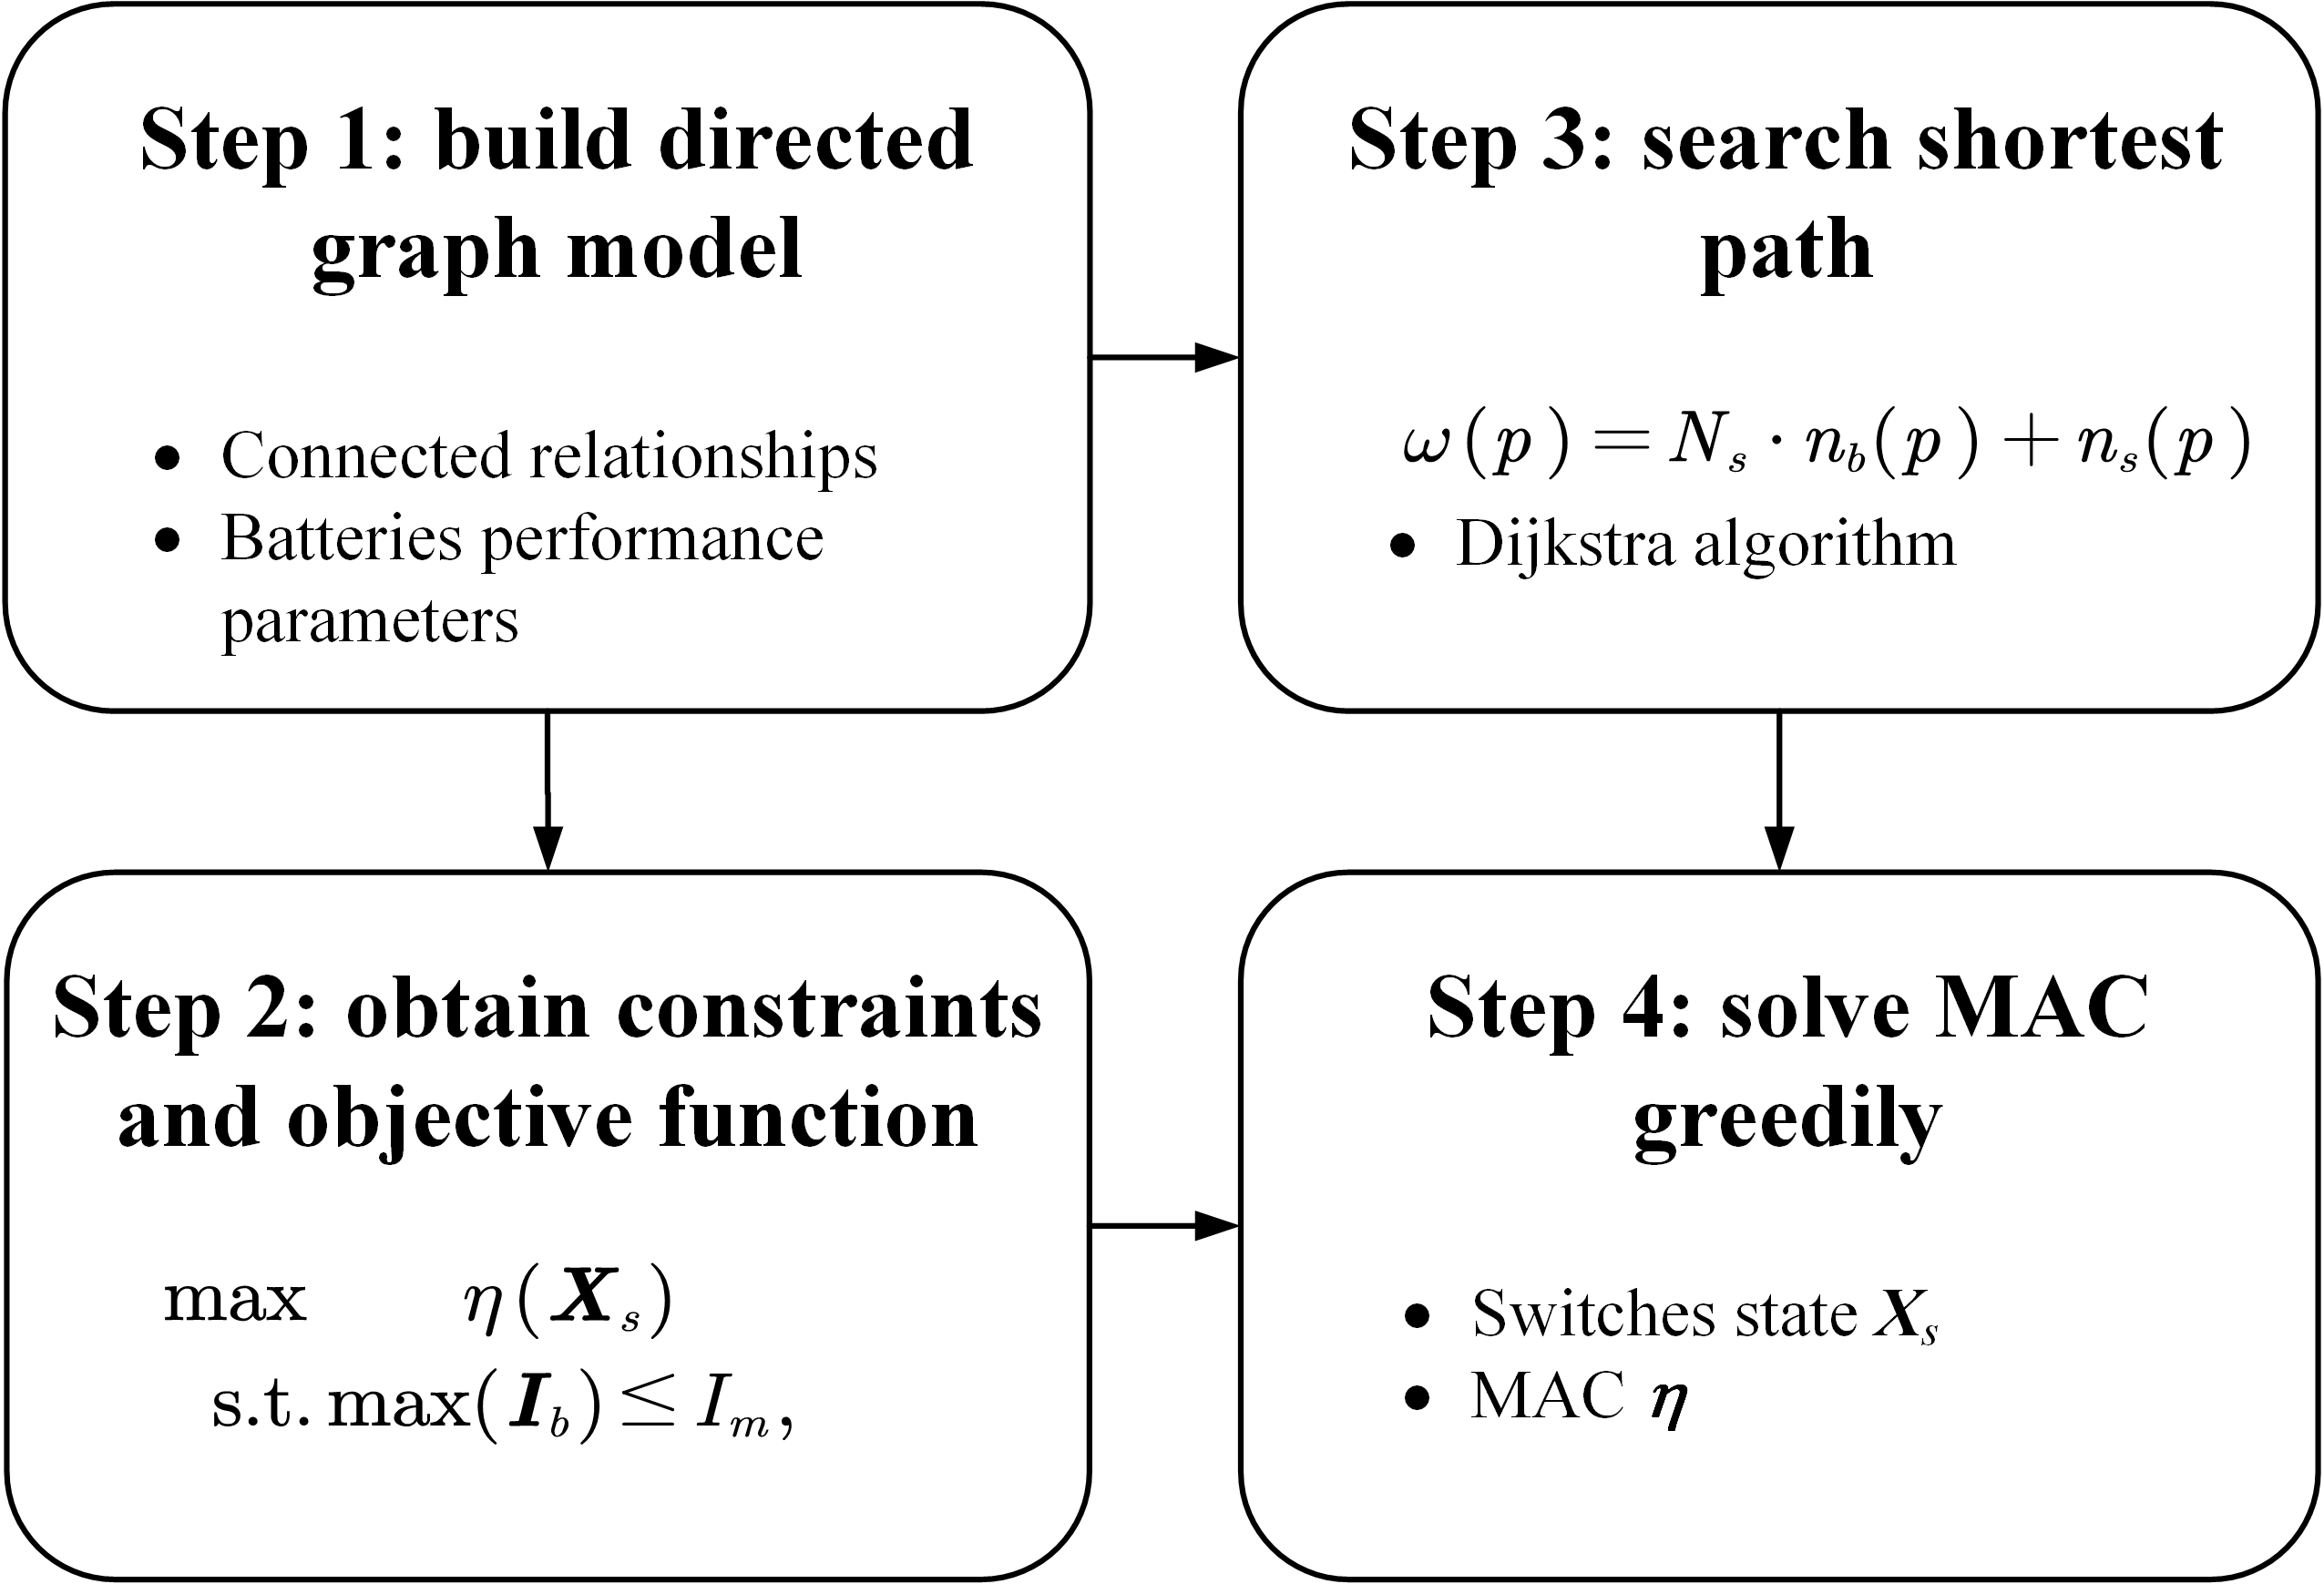
\includegraphics[width=0.8\linewidth]{main.png}
    \caption{
        提出的方法图解,包含四个主要步骤。
    }
    \label{fig:main}
\end{figure}

\subsection{子图}

\begin{figure}[htbp]
    \centering
    \subfloat[] {
        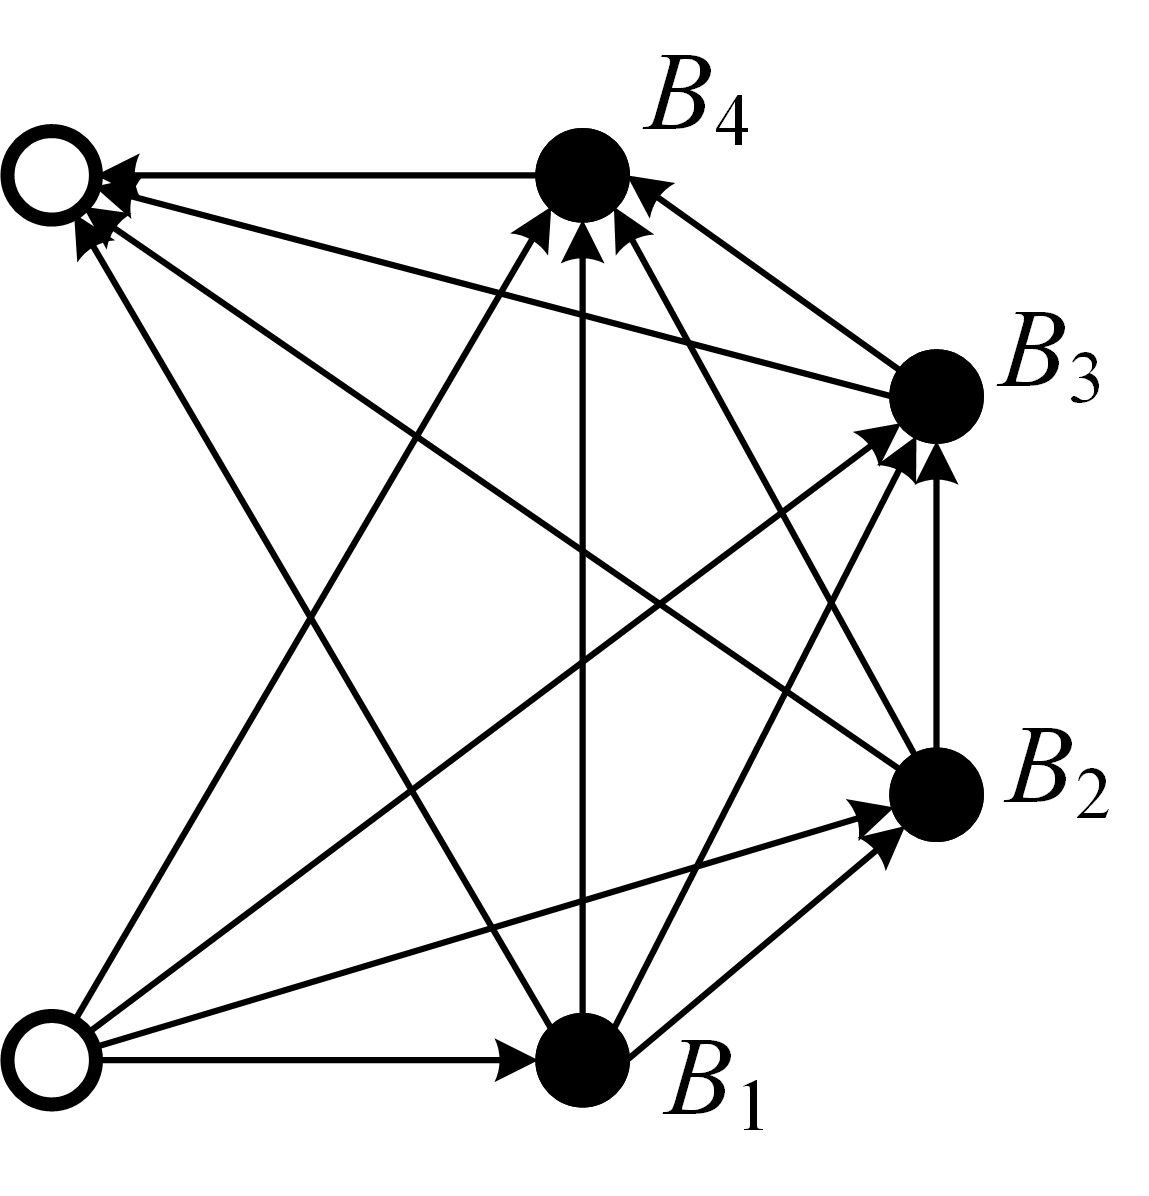
\includegraphics[width=0.31\linewidth]{direct-graph-he.png}
    }\label{fig:direct-graph-he}
    \subfloat[] {
        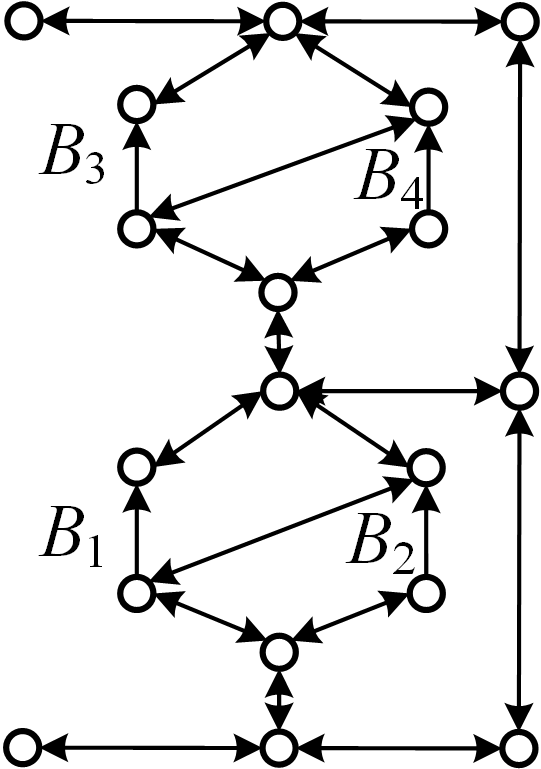
\includegraphics[width=0.23\linewidth]{direct-graph-xu.png}
    }\label{fig:direct-graph-xu}
    \subfloat[] {
        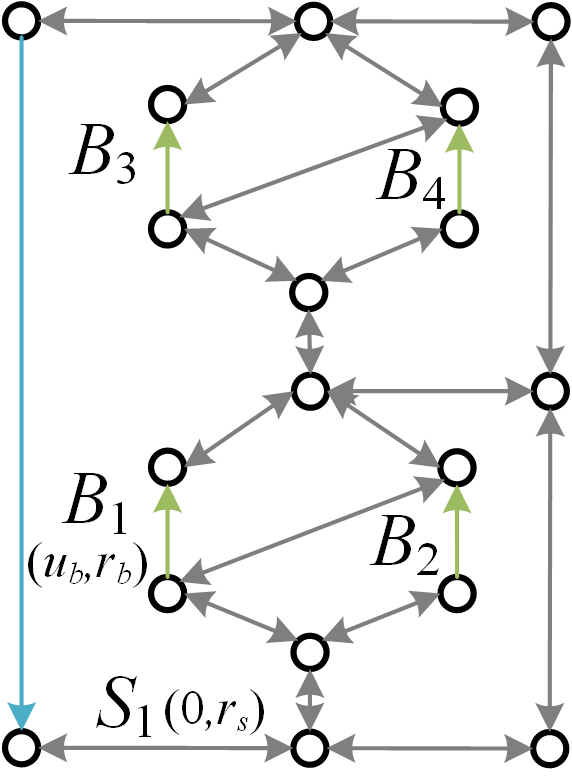
\includegraphics[width=0.24\linewidth]{direct-graph-my.png}
    }\label{fig:direct-graph-my}
    \\
    \subfloat[] {
        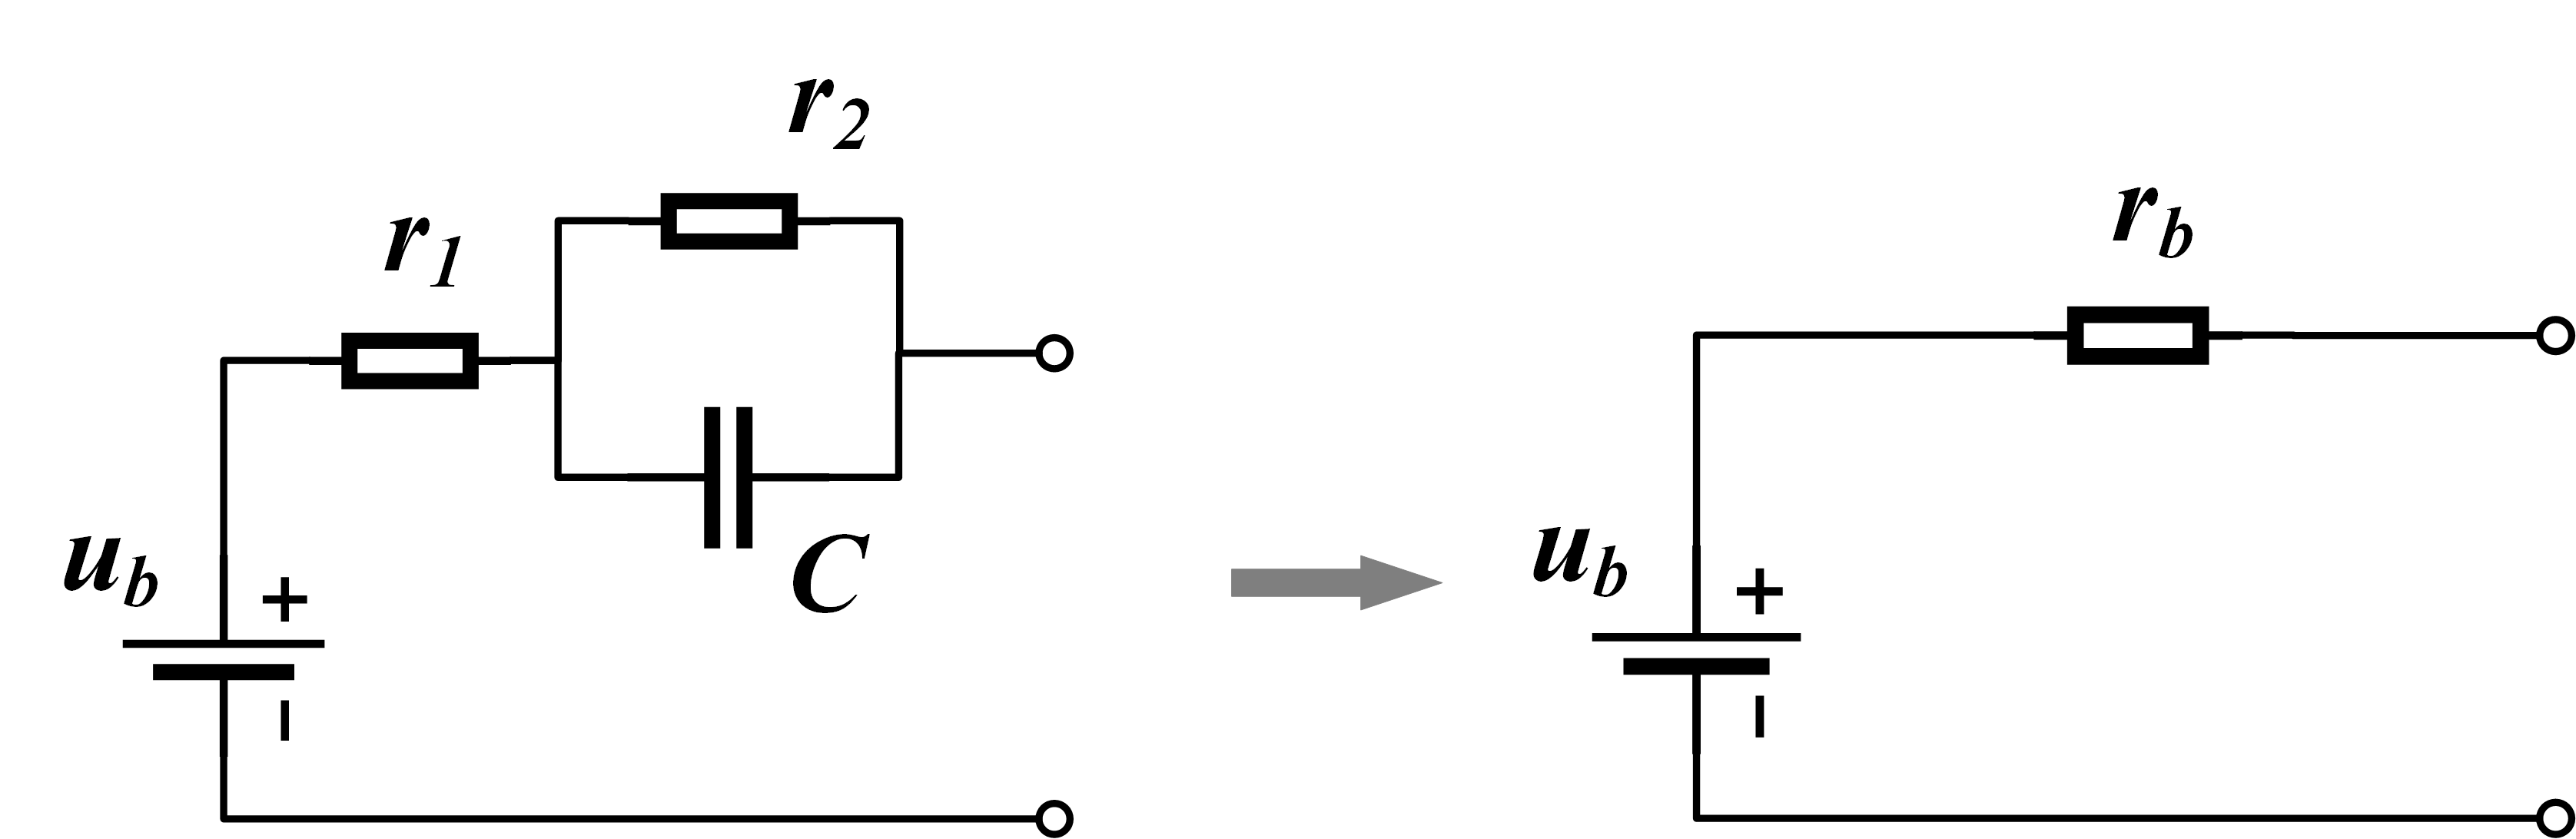
\includegraphics[width=0.8\linewidth]{battery_simple.png}
    }\label{fig:battery-simple}
    \caption{
        定向图模型: (a) He等人的工作 \cite{heExploringAdaptiveReconfiguration2013},(b) 我们之前的工作,(c) 本文提出的改进模型。 (d) 本方法中的电池等效电路图。
    }
    \label{fig:model}
\end{figure}

\paragraph{检查子图的引用}
He等人 \cite{heExploringAdaptiveReconfiguration2013} 提出了一个RBS的抽象定向图模型,其中节点表示电池,边表示配置的灵活性,且每个顶点的权重对应于电池电压(图 \ref{fig:direct-graph-he})。 
...
我们之前提出的定向图模型与He等人的模型显著不同,使用节点表示电池和开关之间的连接,并使用定向边表示电池和开关(图 \ref{fig:direct-graph-xu}),从而实现RBS结构与其定向图模型的一对一对应。
...
图 \ref{fig:direct-graph-my} 显示了本文中使用的改进定向图模型。

\paragraph{检查普通图的引用}
He等人 \cite{heExploringAdaptiveReconfiguration2013} 提出了一个RBS的抽象定向图模型,其中节点表示电池,边表示配置的灵活性,且每个顶点的权重对应于电池电压(图 \ref{fig:model}(a))。 
...
我们之前提出的定向图模型与He等人的模型显著不同,使用节点表示电池和开关之间的连接,并使用定向边表示电池和开关(图 \ref{fig:model}(b)),从而实现RBS结构与其定向图模型的一对一对应。
...
图 \ref{fig:model}(c) 显示了本文中使用的改进定向图模型。

\section{检查公式及其引用}

首先,定向图模型中的拓扑结构以矩阵$\boldsymbol{A}$的形式表示,称为关联矩阵,定义如公式 \eqref{eq:A}:
\begin{align}\label{eq:A}
    a_{kl}=
    \begin{cases}
        1,  & \text{边 $l$ 离开节点 $k$},\\
        -1, & \text{边 $l$ 进入节点 $k$},\\
        0,  & \text{其他情况}.
    \end{cases}
\end{align}
对于由 $N$ 个节点和 $N_b+2N_s+1$ 条定向边组成的定向图,关联矩阵 $\boldsymbol{A}$ 是一个 $N\times(N_b+2N_s+1)$ 的矩阵。 
在该矩阵中,行和列分别表示定向图的节点和边。
通过区分与RBS对应的每一列的组件,$\boldsymbol{A}$ 可以重新写为
\begin{equation}\label{eq:A_bso}
    \boldsymbol{A} =
    \begin{bmatrix}
        \boldsymbol{A}_b & \boldsymbol{A}_s & \boldsymbol{A}_o
    \end{bmatrix},
\end{equation}
其中 $\boldsymbol{A}_b$, $\boldsymbol{A}_s$ 和 $\boldsymbol{A}_o$ 分别是对应于电池、开关和外部负载的子矩阵。
...
类似于公式 \eqref{eq:A_bso},$\boldsymbol{\tilde{A}}$ 可以重新写为
\begin{equation}\label{eq:A_bso_tilde}
    \boldsymbol{\tilde{A}} =
    \begin{bmatrix}
        \boldsymbol{\tilde{A}}_b & \boldsymbol{\tilde{A}}_s & \boldsymbol{\tilde{A}}_o
    \end{bmatrix}.
\end{equation}

\section{检查参考文献}

\bibliographystyle{ieeetr}
\bibliography{../ref}

\end{document}
